\section{Task Log}
\label{sec:task_log}

\begin{figure}[H]
    \hspace*{-2.5cm}
    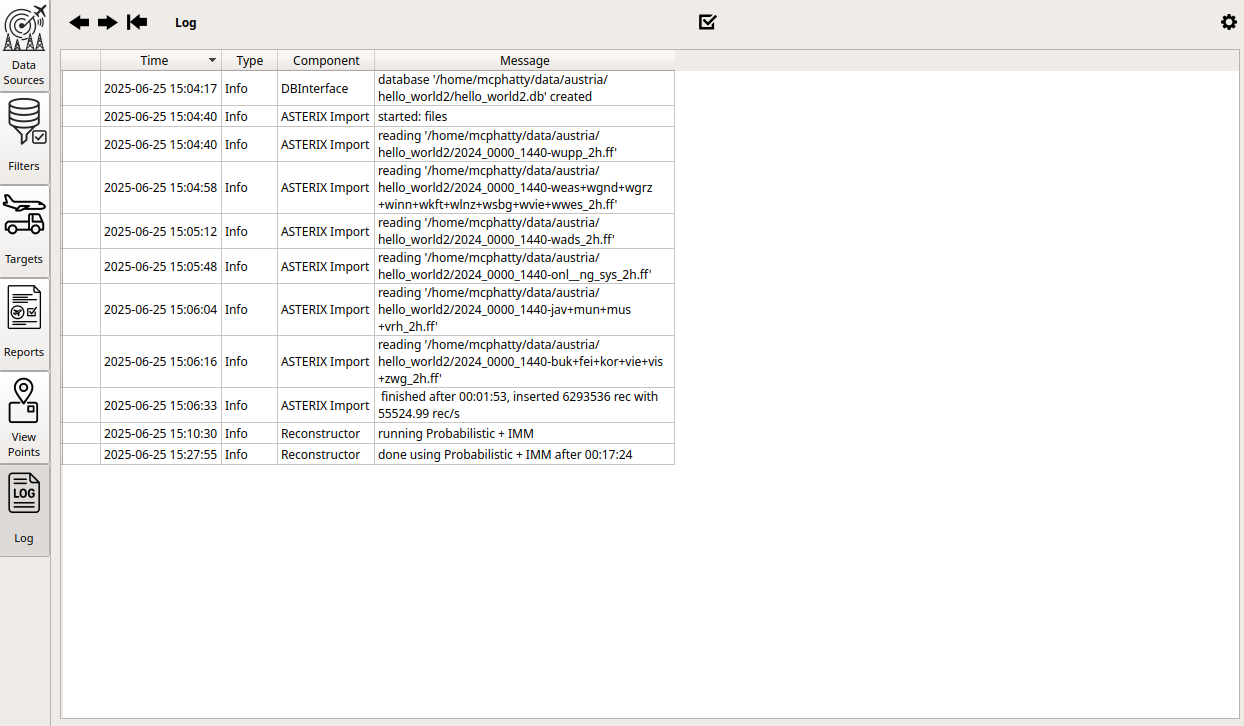
\includegraphics[width=19cm,frame]{figures/task_log.png}
  \caption{Task Log Overview}
\end{figure}

In the 'Task Log' tool, general log messages of importance are created by tasks. Such messages are persisted in the database, and allow an overview of executed tasks, e.g.

\begin{itemize}
  \item DB creation datetime
  \item ASTERIX imports (datetime, filenames, number of target reports)
  \item NMEA GPS trail import
  \item Reconstructor runs
\end{itemize} 
\  \\

This allows for user inspection of error / warning messages without interrupting task execution, as well as inspection of previous task details/results after running (e.g. after automated processing). Error and warning messages are highlighted until accepted by the user.
\\

Please \textbf{note} that further improvements e.g. logging details (additional warning/error messages) will be added in the near future.
